\documentclass{article}
\usepackage{amsmath, amssymb, amsthm}
\usepackage{physics}
\usepackage{float, subcaption, graphicx}

\title{Data-Driven Modeling of Landau Damping by Physics-Informed Neural Networks}
\author{Hunt Feng}
\date{\today}
\begin{document}
    \maketitle

    \begin{abstract}
        In this report, we successfully simulate the Landau damping using finite difference algorithm. The contruction of physics-informed neural network (PINN) is also constructed.
    \end{abstract}

    \section{Introduction}
    Why are we doing this?
    
    \section{Landau Damping}
    Consider a collisionless plasma in the absence of magnetic field, the dynamics of the plasma can be described by the particle distribution $f_s(\mathbf{x},\mathbf{v},t)$, where $s=\{electron, ion\}$ stands for species. The evolution of distribution function is governed by the Vlasov equation,
    \begin{equation} \label{eq:vlasov}
        \pdv{f_s}{t} + \mathbf{v}_s\cdot \grad_\mathbf{r} f_s + \frac{q_s}{m_s}\mathbf{E}\cdot\grad_\mathbf{v} f_s = 0
    \end{equation}
    where $\grad_\mathbf{r}=(\partial_x, \partial_y, \partial_z)$ and $\grad_\mathbf{v}=(\partial_{v_x}, \partial_{v_y}, \partial_{v_z})$. In this report, we consider one-dimensional model in $x-v_x$ space for convenience. 
    
    To complete the system, we introduce the Poisson equation for electric potential,
    \begin{equation} \label{eq:poisson}
        \laplacian\phi = -\rho/\epsilon_0
    \end{equation}
    For convenience, we set the vacuum permittivity $epsilon_0=1$, and the charge density $\rho$ is defined by,
    \begin{equation} \label{eq:charge_density}
        \rho = \sum_s q_sn_s
    \end{equation}
    where the number density $n_s(x,t)$ is defined as
    \begin{equation} \label{eq:number_density}
        n_s(x,t) = \int f_s(x,v_s,t) dv_s
    \end{equation}
    By Gauss's law, we can get electric field,
    \begin{equation}\label{eq:electric_field}
        E(x,t) = -\grad\phi
    \end{equation}
    Equations (\ref{eq:vlasov})-(\ref{eq:electric_field}) forms a complete PDE system. We can investigate the evolution of distribution $f_s(x,v_s,t)$.

    Starting from a plasma at equilibrium. We assume the ions are too heavy to move in a short period of time. Then two perturbation modes is given to the number density of electron. Then the initial number densities of ions and electrons are
    \begin{align} \label{eq:initial_conditions}
        n_e(x,t=0) &= n_0(1 + A_1\cos (k_1x) + A_2\cos (k_2x + \varphi)) \\
        n_i(x,t=0) &= n_0
    \end{align}
    where $n_0$ is the number density of each species at equilibrium. $k_1$ and $k_2$ are the wavenumbers of the two perturbation modes, $A_1$ and $A_2$ are their amplitudes, and $\varphi$ is a random phase.

    The result of simulation is shown below.

    \begin{figure} [H]
        \centering
        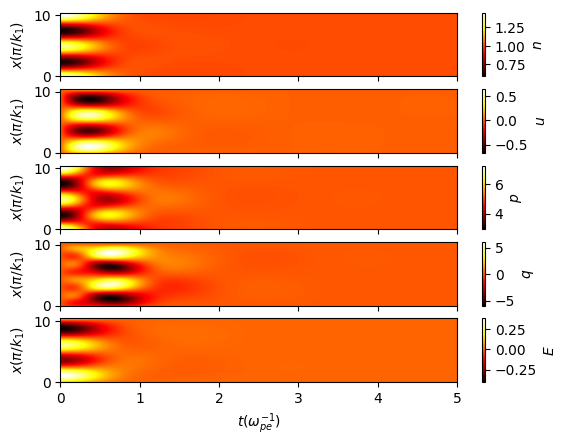
\includegraphics[width=0.7\textwidth]{img/simulation_fields.png}
        \label{fig:simulation_fields}
    \end{figure}

    \begin{figure} [H]
        \centering
        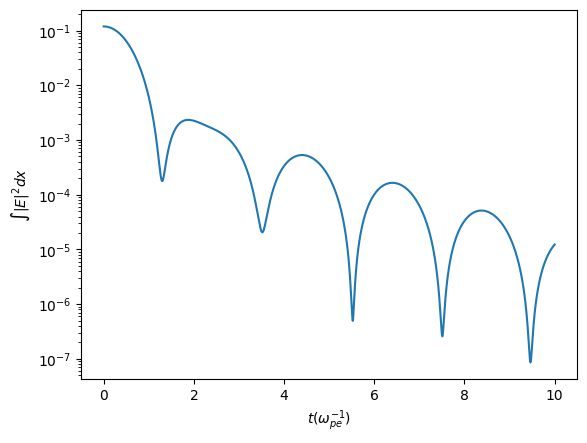
\includegraphics[width=0.7\textwidth]{img/simulation_energy.png}
        \label{fig:simulation_energy}
    \end{figure}


    \section{Physics-Informed Nueral network (PINN)}
    
    \section{Methodology}
    \subsection{Data Preparation}

    \subsection{Construction of PINN}

    \subsection{Training the PINN}

    \section{Result}


    \nocite{*}
    \bibliography{references}
    \bibliographystyle{plain}
\end{document}